\section{Results}
\label{sec:results}

\subsection{Cohort attrition}
The initial MIMIC-IV corpus contained 5{,}862{,}940 radiology reports from 237{,}425 patients.  
After removal of duplicate documents, 5{,}861{,}692 reports remained. Filtering to inpatient and outpatient encounters with supported imaging modalities (\texttt{MRI Brain}, \texttt{CT Brain}, \texttt{CT Chest}, \texttt{CT Pelvis}, \texttt{CT Cervical Spine}, \texttt{Ultrasound}) yielded 338{,}491 reports from 101{,}353 patients.  
A stratified random sample of 500 reports was used for readability and bias assessment.

\subsection{Readability score analysis}
We evaluated readability differences between privileged and underprivileged demographic groups across four indices—\texttt{SMOG, FKG, GUNN, and CLI}—for all models.  
Differences are reported as $\Delta = \text{Privileged} - \text{Underprivileged}$.

\begin{figure}[!ht]
    \centering
    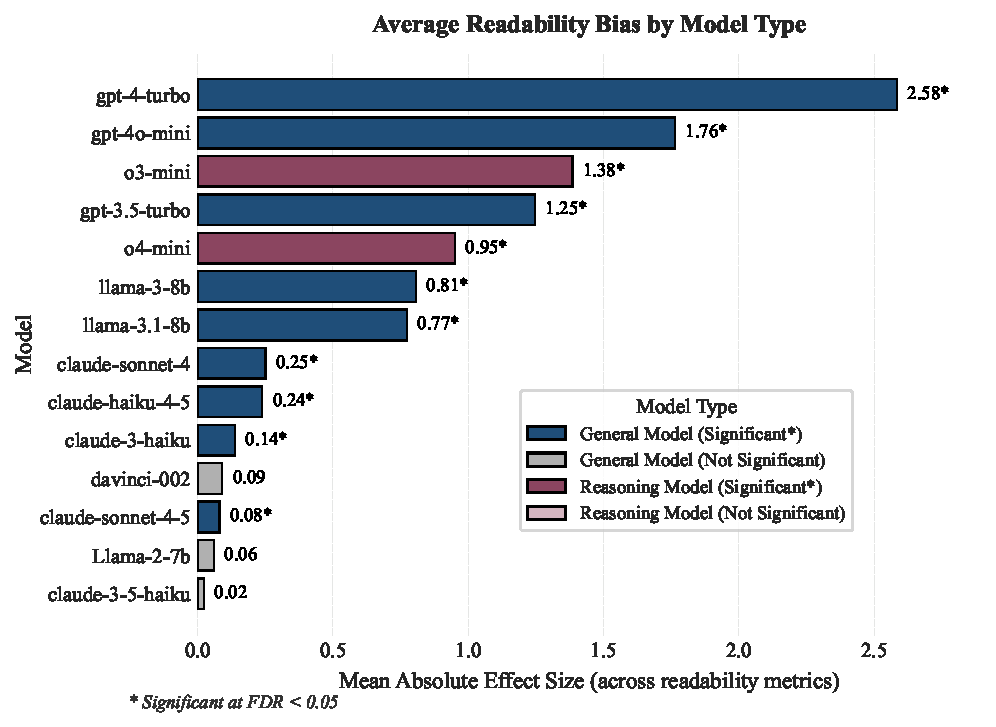
\includegraphics[width=\textwidth]{figures/FigureReadabilityBias.pdf}
    \caption{Readability differences between privileged and underprivileged demographic groups across four readability indices (FKG, SMOG, GUNN, CLI) for various LLM models.}
    \label{fig:readability_bias}
\end{figure}

\subsubsection{Overall patterns across LLM families}
Across modern LLMs, privileged-group outputs consistently showed higher readability grades across all four indices.  
Early-generation models exhibited minimal or statistically nonsignificant differences across metrics (e.g., \texttt{Llama-2-7b}: $\Delta_{\mathrm{CLI}} = 0.297$, $p = 0.0599$; $\Delta_{\mathrm{FKG}} = -0.023$, $p = 0.98$).  
In contrast, contemporary instruction- and reasoning-tuned models demonstrated substantial and statistically significant gaps.

\subsubsection{Metric-specific findings}
\begin{table}[!ht]
    \centering
    \begin{tabular}{lcccc}
        \toprule
        \textbf{Model} & \textbf{FKG} & \textbf{SMOG} & \textbf{GUNN} & \textbf{CLI} \\
        \midrule
        \textit{Early-generation models} & & & & \\
        Llama-2-7b & $-0.023$ & $0.019$ & $0.002$ & $0.297$ \\
        davinci-002 & $-0.331$ & $0.065$ & $-0.314$ & $0.501$ \\
        \midrule
        \textit{Intermediate-generation models} & & & & \\
        gpt-3.5-turbo & $0.958^{***}$ & $0.893^{***}$ & $1.153^{***}$ & $1.114^{***}$ \\
        llama-3-8b-instruct & $0.913^{***}$ & $0.821^{***}$ & $1.127^{***}$ & $1.197^{***}$ \\
        \midrule
        \textit{Advanced models} & & & & \\
        GPT-4-turbo & $1.669^{***}$ & $1.413^{***}$ & $1.976^{***}$ & $1.499^{***}$ \\
        gpt-4o-mini & $0.977^{***}$ & $0.783^{***}$ & $1.161^{***}$ & $0.816^{***}$ \\
        o3-mini & $1.019^{***}$ & $0.837^{***}$ & $1.204^{***}$ & $0.994^{***}$ \\
        o4-mini & $1.278^{***}$ & $1.150^{***}$ & $1.608^{***}$ & $1.239^{***}$ \\
        llama-3.1-8b-instruct & $1.280^{***}$ & $1.100^{***}$ & $1.432^{***}$ & $1.536^{***}$ \\
        \midrule
        \textit{Claude models} & & & & \\
        claude-3-haiku & $-0.010$ & $0.107$ & $0.153$ & $0.163$ \\
        claude-3-5-haiku & $-0.752$ & $-0.203$ & $-0.761$ & $0.039$ \\
        claude-haiku-4-5 & $-0.477$ & $0.160$ & $-0.360$ & $0.497^{***}$ \\
        claude-sonnet-4 & $-0.168$ & $0.345$ & $-0.083$ & $0.356^{***}$ \\
        claude-sonnet-4-5 & $-0.405$ & $-0.091$ & $-0.361$ & $0.108$ \\
        \bottomrule
    \end{tabular}
    \caption{Readability differences between privileged and underprivileged groups across LLM models and metrics. Values show $\Delta = \text{Privileged} - \text{Underprivileged}$. $^{***}p < 10^{-6}$. Positive values indicate higher readability grades (more complex text) for privileged groups. Negative values indicate higher complexity for underprivileged groups.}
    \label{tab:readability_metrics}
\end{table}

\paragraph{FKG.}
Differences ranged from near-zero in early models to large and statistically significant gaps in advanced systems.  
\texttt{GPT-4-turbo} showed the largest difference ($\Delta = 1.669 \pm 0.683$, $d = 2.443$, $p < 10^{-6}$).  
Other high-performing models, including \texttt{gpt-4o-mini}, \texttt{o3-mini}, \texttt{o4-mini}, and the Llama-3 family, also demonstrated significant differences ($\Delta = 0.913$--$1.280$, all $p < 10^{-6}$).  
Older models (\texttt{davinci-002}, \texttt{Llama-2-7b}) showed negligible or inconsistent effects.

\paragraph{SMOG.}
SMOG differences followed the same trend, with small effects for legacy models (e.g., \texttt{Llama-2-7b}: $\Delta = 0.019$, $p = 0.76$) and large, statistically significant differences in advanced models.  
\texttt{GPT-4-turbo} again exhibited the largest gap ($\Delta = 1.413 \pm 0.562$, $d = 2.514$, $p < 10^{-6}$).  
\texttt{gpt-3.5-turbo}, \texttt{gpt-4o-mini}, and the Llama-3 series also showed substantial differences ($\Delta = 0.783$--$1.100$, all $p < 10^{-6}$).

\paragraph{GUNN.}
GUNN yielded the largest absolute differences among the four metrics.  
\texttt{GPT-4-turbo} produced the highest mean difference ($\Delta = 1.976 \pm 0.779$, $d = 2.536$, $p < 10^{-6}$).  
\texttt{gpt-4o-mini}, \texttt{o3-mini}, \texttt{o4-mini}, and Llama-3 variants also demonstrated consistent gaps ($\Delta = 1.127$--$1.608$, all $p < 10^{-6}$).  
Earlier models showed negligible differences (e.g., \texttt{Llama-2-7b}: $\Delta = 0.002$, $p = 0.517$).

\paragraph{CLI.}
Significant effects were observed for all advanced models, including \texttt{GPT-4-turbo} ($\Delta = 1.499 \pm 0.527$, $d = 2.845$, $p < 10^{-6}$), \texttt{gpt-4o-mini} ($\Delta = 0.816 \pm 0.467$, $d = 1.75$, $p < 10^{-6}$), \texttt{o3-mini}, \texttt{o4-mini}, and the Llama-3 series.  
Early models again showed small or nonsignificant effects (e.g., \texttt{claude-3-5-haiku}: $\Delta = 0.039$, $p = 0.289$).

\subsubsection{Model progression trends}
A capability-aligned pattern was observed across model generations.

\paragraph{Early-generation models.}
\texttt{Llama-2-7b} and \texttt{davinci-002} showed small and statistically nonsignificant differences across all metrics.

\paragraph{Intermediate-generation models.}
\texttt{gpt-3.5-turbo} and \texttt{Llama-3-8B} exhibited moderate differences across metrics, with significant effects across all readability indices for \texttt{gpt-3.5-turbo} (e.g., $\Delta_{\mathrm{FKG}} = 0.958$, $d = 1.18$, $p < 10^{-6}$).

\paragraph{Advanced models.}
\texttt{GPT-4-turbo}, \texttt{gpt-4o-mini}, \texttt{o3-mini}, \texttt{o4-mini}, and \texttt{Llama-3.1-8B} demonstrated large, statistically significant differences across all readability indices, typically ranging from $\Delta \approx 0.8$ to $2.0$, with effect sizes often exceeding $d>1.5$.

\subsection{SEAT analysis}
SEAT results supported the readability findings.  
Early-generation models showed negligible embedding-level differences (e.g., \texttt{Llama-2-7b}: $d = -0.018$, $p = 0.65$).  
Modern models exhibited significant associations of privileged-group embeddings with more expert-like language.  
\texttt{GPT-4-turbo} showed the largest embedding bias ($d = -0.629$, $p < 10^{-6}$), followed by \texttt{gpt-4o-mini} ($d = -0.458$, $p < 10^{-6}$), \texttt{o3-mini} ($d = -0.437$, $p < 10^{-6}$), and \texttt{o4-mini} ($d = -0.360$, $p < 10^{-6}$).  
The Llama-3 family also demonstrated consistent medium-size effects ($d = -0.311$ to $-0.355$; all $p < 10^{-6}$).

Overall, readability-based and embedding-based analyses aligned, indicating that newer model generations consistently produce more complex text for privileged groups across metrics and evaluation modalities.

\subsection{Demographic Parity Analysis}

\paragraph{Percentile-Based Demographic Parity.}
Privileged groups demonstrated higher representation in the high-complexity tail of the readability distribution.  
For the top-20\% threshold, privileged vs.\ underprivileged selection rates were $0.2209$ and $0.1821$ ($\Delta = 0.0389$), respectively.  
For the top-30\% threshold, the disparity increased ($0.3428$ vs.\ $0.2599$; $\Delta = 0.0829$).  
These findings indicate moderate tail-risk disparity, with privileged groups more likely to receive explanations in the highest-complexity percentile bands.

\paragraph{Distributional Parity (Wasserstein + KL).}
Global distributional differences between groups were substantial.  
The Wasserstein distance between privileged and underprivileged readability distributions was $W = 0.6073$, indicating a pronounced shift in distributional mass.  
KL divergence values further confirmed asymmetric distributional behavior (KL$_{\text{priv}\rightarrow\text{unpriv}} = 0.0896$, KL$_{\text{unpriv}\rightarrow\text{priv}} = 0.0964$).  
Together, these metrics demonstrate that privileged and underprivileged groups receive systematically different output complexity profiles.

\paragraph{Counterfactual Demographic Parity.}
Counterfactual analysis revealed strong evidence of causal demographic bias.  
When demographic descriptors were varied while holding report content fixed, the privileged demographic variant produced higher readability scores in $64.8\%$ of matched report pairs (CDP = $0.648$).  
This indicates that demographic attributes alone can induce significant shifts in explanation complexity, independent of underlying clinical content.